\section{Statistical analysis of experiment 1}\label{sub:Stat1}\todo{Split into expectations and result}

In this section the various statistical methods covered in \cref{subsec:correlation} and \cref{subsec:distribution} will be used to analyses the data. The initial step is to verify if the data is normally distributed as it has an effect on which statistical methods can be used to analyze the data. To do this the Shapiro-Wilk test will be used to check if the data is normally distributed, to see which statistical methods should be utilized. Then the MannWhitney U Test will test if they are from the same population or not, and finally the correlation between the different measure will be calculated and analyzed.

\subsection{Normal distribution}\label{subsec:NormalDist1}

The Sharpiro Wilk test will be used to test if the data is normally distributed, this is important as is effects which statistical methods can be applied to the data correctly as covered in \cref{subsec:distribution}. 

\paragraph{Expectations}
For the Sharpiro Wilk test the expectations are that the some of the data will not be normally distributed, this assumption is mostly based on the findings by\cite{Koedijk2022diff}. We expect most of the data to either be normally distributed or close to, while having some outliers that behave differently.

\paragraph{Result}
The results show that the data for the different DUTs are not all normally distributed, though the majority is.
\begin{table}[]
    \begin{tabular}{||c|c|c|c|c|c||}
    &\textbf{TestCaseIdle}&\textbf{BinaryTrees}&\textbf{FannkuchRedux}&\textbf{Nbody}&\textbf{Fasta}\\ [0.5ex] \hline\hline
    \textbf{IntelPowerGadget}&0.0004&0.3685&0.0007&0.0&0.0809\\
    \textbf{HardwareMonitor}&0.0&0.0033&0.088&0.0&0.0002\\
    \textbf{E3}&0.9307&0.2229&0.0&0.0966&0.0002\\
    \textbf{RAPL}&0.0152&0.0311&0.0&0.0&0.0007\\ \hline
    \end{tabular}
    \caption{Here the various values for p using the Shapiro Wilk test for the testcases on the Surface Book}
    \label{tab:NormDistSurfB}
\end{table}½
As can be seen in \cref{tab:NormDistSurfB}, the majority of the results are normally distributed given $P = 0.05$\todo{is 0.05 mentioned somewhere}. This is however not the case for all results, which is why the statistical methods able to handle non-normally distributed data is used. This in line with what we expected based on the literature.

\subsection{Independence Test}\label{subsec:independence1}
To Test the independence of the data either the T-test or the MannWhitney U Test can be used depending on the distribution of the data. It was found in \cref{subsec:NormalDist1}, that the data was not normally distributed. Thus the MannWhitney U Test will have to be used instead as it is non-parametric independence test, allowing a comparison of the different measurement foreach of the test cases to check if they are are independent from each other. The null hypothesis $H_0$ for the Mann-Whitney U test is defined as:

\begin{quote}
    \textit{In the population, the sum of the rankings in the two groups does not differ.}
\end{quote}

\paragraph{Expectations}
The expectation is that $H_0$ can be rejected in all cases as each of the measurement are obtained independently from each other and should not influence each other as found in \cref{subsec:exp_r3}. Thus the results should in most cases be close to zero.

\paragraph{results}
The results from the FannkuchRedux test case can be seen below, where the results for the remaining test cases can be found in the appendix.\todo{cref til dem}
\begin{figure}
  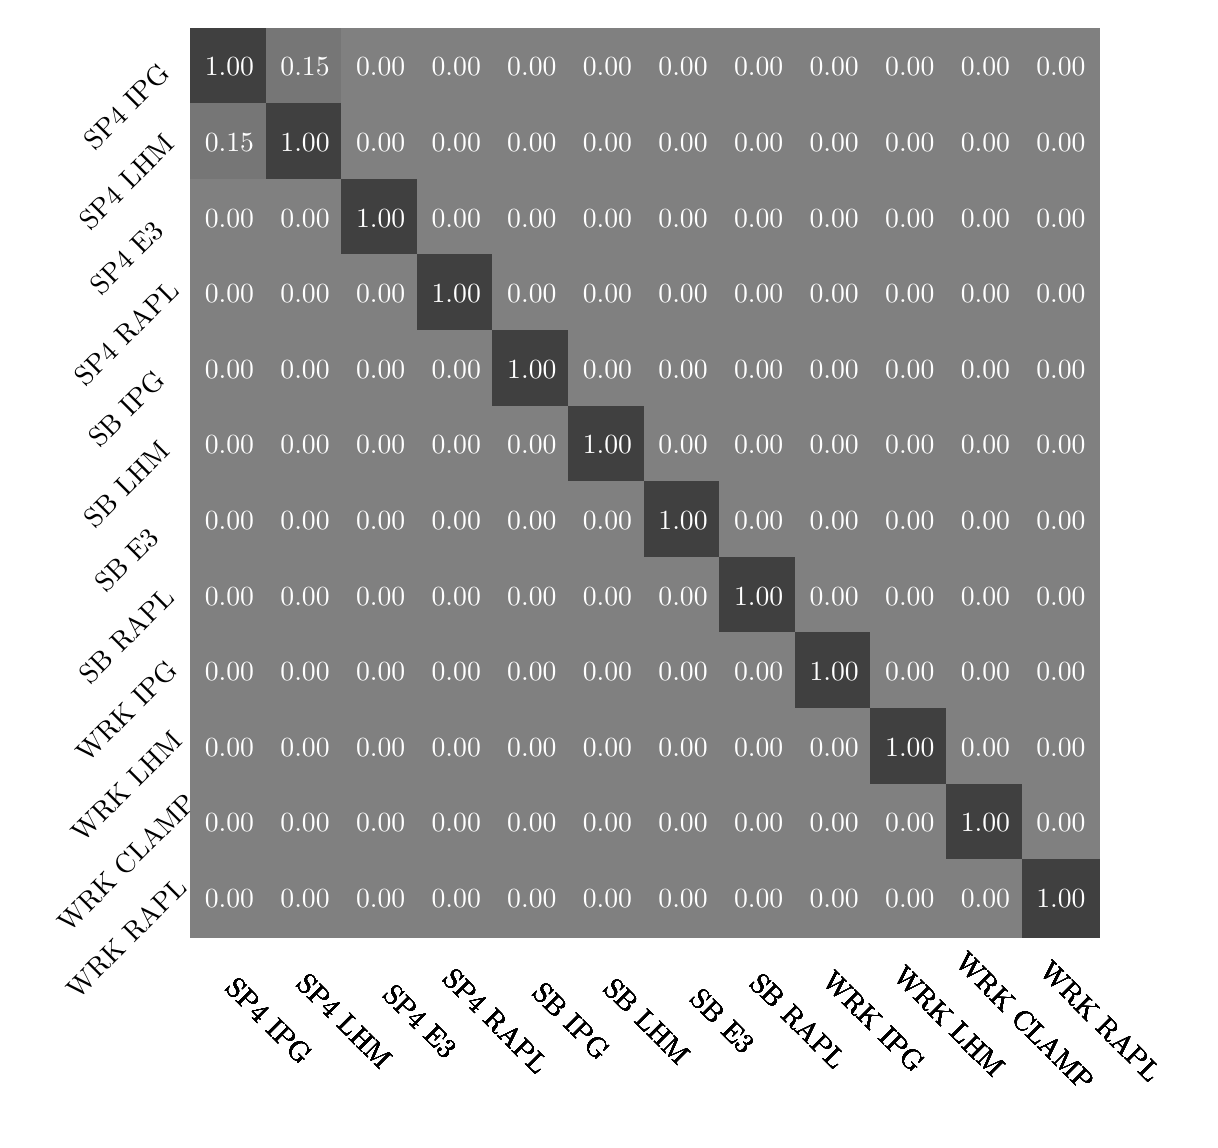
\begin{tikzpicture}[scale=0.6]
    \foreach \y [count=\n] in {{1.00, 0.15, 0.00, 0.00, 0.00, 0.00, 0.00, 0.00, 0.00, 0.00, 0.00, 0.00},{0.15, 1.00, 0.00, 0.00, 0.00, 0.00, 0.00, 0.00, 0.00, 0.00, 0.00, 0.00},{0.00, 0.00, 1.00, 0.00, 0.00, 0.00, 0.00, 0.00, 0.00, 0.00, 0.00, 0.00},{0.00, 0.00, 0.00, 1.00, 0.00, 0.00, 0.00, 0.00, 0.00, 0.00, 0.00, 0.00},{0.00, 0.00, 0.00, 0.00, 1.00, 0.00, 0.00, 0.00, 0.00, 0.00, 0.00, 0.00},{0.00, 0.00, 0.00, 0.00, 0.00, 1.00, 0.00, 0.00, 0.00, 0.00, 0.00, 0.00},{0.00, 0.00, 0.00, 0.00, 0.00, 0.00, 1.00, 0.00, 0.00, 0.00, 0.00, 0.00},{0.00, 0.00, 0.00, 0.00, 0.00, 0.00, 0.00, 1.00, 0.00, 0.00, 0.00, 0.00},{0.00, 0.00, 0.00, 0.00, 0.00, 0.00, 0.00, 0.00, 1.00, 0.00, 0.00, 0.00},{0.00, 0.00, 0.00, 0.00, 0.00, 0.00, 0.00, 0.00, 0.00, 1.00, 0.00, 0.00},{0.00, 0.00, 0.00, 0.00, 0.00, 0.00, 0.00, 0.00, 0.00, 0.00, 1.00, 0.00},{0.00, 0.00, 0.00, 0.00, 0.00, 0.00, 0.00, 0.00, 0.00, 0.00, 0.00, 1.00},} {
    % column labels
    \foreach \a [count=\n] in {SP4 IPG,SP4 LHM,SP4 E3,SP4 RAPL,SB IPG,SB LHM,SB E3,SB RAPL,WRK IPG,WRK LHM,WRK CLAMP,WRK RAPL} {
      \node[minimum size=10mm, xshift=0.5cm, rotate=-45] at (\n*1.6, -21.8) {\a};
    }
    % heatmap tiles
    \foreach \x [count=\m] in \y {
      \pgfmathsetmacro{\xa }{(\x + 1) / 2 * 100}
      \node[fill=darkgray!\xa!lightgray, minimum size=10mm, text=white, font={\normalsize}] at (\m*1.6,-\n*1.6) {\x};
    }
  }
    % row labels
    \foreach \a [count=\i] in {SP4 IPG,SP4 LHM,SP4 E3,SP4 RAPL,SB IPG,SB LHM,SB E3,SB RAPL,WRK IPG,WRK LHM,WRK CLAMP,WRK RAPL} {
      \node[minimum size=10mm, xshift=-0.35cm, yshift=-0.5cm, rotate=45] at (0,-\i*1.6) {\a};
    }
  \end{tikzpicture}
  \caption{Here the results for the FannkuchRedux on the Mann Whitney U Test can be seen. The Range in $0 - 1$}
  \label{tab:HeatFannkuchRedux}
  \end{figure} 
As can be seen in \cref{tab:HeatFannkuchRedux}, the majority of the values are below $p = 0.05$, meaning that we can confidently reject the null hypotheses. The only cases where $H_0$ cannot be rejected is SP4 LHM and SP4 IPG. This aligns with the expectations that the samples are independent of each other in the majority of cases.


\subsection{Correlation}\label{subsec:correlation1}
In this section the correlation between the data will be calculated, to do this the Kendal Tau correlation coefficients will be used, because it was found in \cref{subsec:NormalDist1}, that the data was not normally distributed. To test the results from the Test cases with Kendall tau the following data is preprocessed in the following manner. When using the Kendall Tau Correlation, the test case results for each of the DUTs were appended to each other and sorted based on the test case, an example of which can be seen in \cref{tab:RainBowGraph}.

\input{tabels/experiment_results/exp_one/StatQuest/stats.tex}
In \cref{tab:RainBowGraph} the background represents which test case the data point is a measurement of and these are then used to calculate the correlation as seen in \cref{tab:correlationWork} and \cref{tab:HeatFasta}.

\paragraph{Expectations}
The expectations are that all of the measurement instrument will positively correlated with each other. Though to what degrees this positive correlations will be present is unknown though higher correlations would generally be more indicative of valid measurements, as it show the measurement instruments agreeing.

\paragraph{Result}
Here the results from the correlations can be seen for the different DUTs and the different measurement instruments. The results for the workstation can be seen in \cref{tab:correlationWork}, the Surface4Pro in \cref{tab:correlationSurfP} and the SurfaceBook in \cref{tab:CompbinedSurfB}
\begin{figure}
\centering
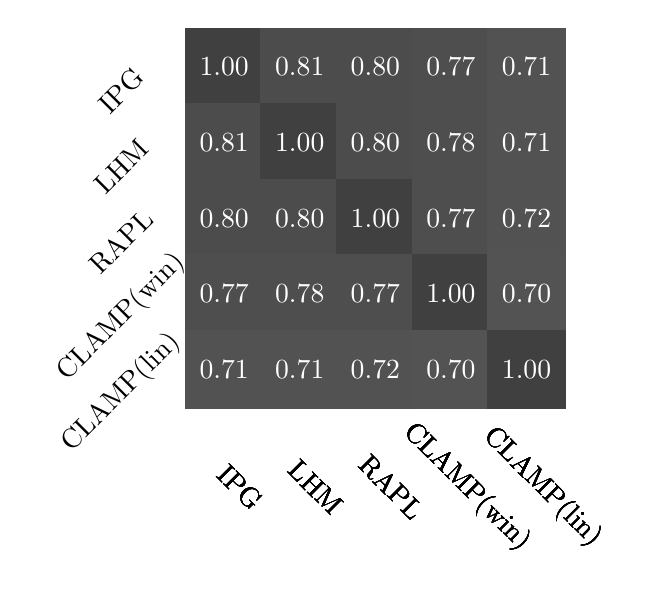
\begin{tikzpicture}[scale=0.6]
  \foreach \y [count=\n] in {{1.00, 0.81, 0.80, 0.77, 0.71},{0.81, 1.00, 0.80, 0.78, 0.71},{0.80, 0.80, 1.00, 0.77, 0.72},{0.77, 0.78, 0.77, 1.00, 0.70},{0.71, 0.71, 0.72, 0.70, 1.00},} {
  % column labels
  \foreach \a [count=\n] in {IPG,LHM,RAPL,CLAMP(win),CLAMP(lin)} {
    \node[minimum size=10mm, xshift=0.2cm, rotate=-45] at (\n*1.6, -10.50) {\a};
  }
  % heatmap tiles
  \foreach \x [count=\m] in \y {
    \pgfmathsetmacro{\xa }{(\x + 1) / 2 * 100}
    \node[fill=darkgray!\xa!lightgray, minimum size=10mm, text=white, font={\normalsize}] at (\m*1.6,-\n*1.6) {\x};
  }
}
  % row labels
  \foreach \a [count=\i] in {IPG,LHM,RAPL,CLAMP(win),CLAMP(lin)} {
    \node[minimum size=10mm, xshift=-0.35cm, yshift=-0.3cm, rotate=45] at (0,-\i*1.6) {\a};
  } 
\end{tikzpicture}
\caption{This heat map represents Correlation coefficients between the different measuring instruments -1 to 1 on the Workstation}
\label{tab:correlationWork}
\end{figure}
\input{tabels/experiment_results/exp_one/StatQuest/Correlation/CompbinedSurfBP.tex}
These results match our expectations as all of the correlations are a positive. A more in depth analysis of these results will be conducted in \cref{subsec:ResultStat1}

\subsection{Results}\label{subsec:ResultStat1}
Here the results from \cref[subsec:NormalDist1, subsec:independence1,subsec:correlation1], will be analyses more in depth and using it to answer our research questions \textbf{RQ2},\textbf{RQ3} and \textbf{RQ4}.

\paragraph{RQ2}
When comparing the measurement instrument to each other.
The correlations coefficients found in \cref{subsec:correlation1}, can be used. When evaluating the results, the scale presented by Guildford in \cite[219]{guilford1950fundamental} to evaluate correlation can be used. 
\begin{itemize}
    \item $<.20$: Slight; almost negligible relationship
    \item $.20-.40$: Low correlation; definite but small relationship
    \item $.40-.70$: Moderate correlation; substantial relationship
    \item $.70-.90$: High Correlation; marked relationship
    \item $.90-1$: Very high correlation; very dependable relationship
\end{itemize}
Using this scale we can evaluate the correlation between the different measuring instruments. Looking across the different DUTs we can calculate average correlation between each of the measuring instruments. When comparing the correlation between the different measuring instruments across all DUTs, the correlation is as following:

$$IPG|LHM = (0.68+0.81+0.69)/3 = 0.726$$
$$IPG|RAPL = (0.30+0.42+0.80)/3 = 0.506$$
$$LHM|RAPL = (0.80+0.39+0.21)/3 = 0.466$$

Now, the average correlation between the different software measuring instruments against the clamp will be calculated. This is done for only the workstation, as the the clamp was only used on this DUT.

$$IPG|Clamp = (0.77+0.71)/2 = 0.74$$
$$LHM|Clamp = (0.78+0.71)/2 = 0.745$$
$$RAPL|Clamp = (0.77+0.72)/2 = 0.745$$

Similarly, the average correlation between the different measuring instruments from the DUTs with a battery can be calculated, to see how they are correlated with E3.

$$IPG|E3 = (0.63+0.61)/2 = 0.62$$
$$LHM|E3 = (0.65+0.64)/2 = 0.645$$
$$RAPL|E3 = (0.24+0.49)/2 = 0.365$$

Looking at these numbers and evaluating them on the Guildford scale, we can see that IPG|LHM, IPG|Clamp and RAPL|Clamp all are highly correlated and marked relationships, while LHM|RAPL, LHM|RAPL,IPG|E3 and LHM|E3 has a substantial relationships. The lowest correlation between the measurements was found with RAPL|E3 which are a low on correlation.
\paragraph{RQ3}
In regards to the different operating system and how these effect the results it can be seen that these are are differences between the measurements conducted on Linux and Windows.
Looking at the coefficients for RAPL and CLAMP(lin) int can be seen that they are generally less correlated with the other measurement instruments Then there Windows counter part. This can be clearly seen when calculating the average coefficients for each of the instruments across the different DUTs.
\begin{itemize}
    \item \textbf{Windows}
    \begin{itemize}
        \item $IPG = 0.642$ %0.81+0.80+0.77+0.71+0.68+0.30+0.63+0.69+0.42+0.61
        \item $LHM = 0.635$ %0.81+0.8+0.78+0.71+0.68+0.2+0.65+0.69+0.39+0.64
        \item $CLAMP(win) = 0.755$ %0.77+0.78+0.77+0.70
        \item $E3 = 0.543$ %0.63+0.65+0.61+0.64+0.24+0.49
    \end{itemize}
    \item \textbf{Linux}
    \begin{itemize}
        \item $CLAMP(lin) = 0.71$ %0.71+0.71+0.72+0.70
        \item $RAPL = 0.513$ %0.80+0.80+0.77+0.72+0.3+0.2+0.24+0.42+0.39+0.49
    \end{itemize}
\end{itemize}
Looking at these number it can be seen that linux that Rapl and the hardware measurements on linux are generally less correlated with the rest of the measurement instruments. This does make sense as they are different OSs and would be expected to have different power consumption.

\paragraph{RQ4}
comparing the different DUTs in a similar manner i can be found that there are significant differences between how correlated the measurement instruments are on each DUT.
\begin{itemize}
    \item \textbf{Workstation}
    \begin{itemize}
        \item Average coefficients: $0.757$%
    \end{itemize}
    \item \textbf{Surface 4 Pro}
    \begin{itemize}
        \item Average coefficients: $0.540$%0.69+0.42+0.61+0.39+0.64+0.49
    \end{itemize}
    \item \textbf{Surface Book}
    \begin{itemize}
        \item Average coefficients: $0.450$ %0.68+0.30+0.63+0.20+0.65+0.24
    \end{itemize}
\end{itemize}
When comparing the different DUTs it can be seen that the measurement instruments are more correlated with each other on the Workstation than on the two laptops. Comparing the two laptops it can be seen that the Surface Book as a significantly lower coefficients than the Surface 4 Pro. Looking more close at the number they are very similar in all cases except for Rapl where the surface book performance much worse. Comparing the average Rapl coefficients between the two DUTs results in a stark difference.
\begin{itemize}
    \item Surface book:$AvgRAPL = 0.246$
    \item Surface 4 Pro:$AvgRAPL = 0.433$
\end{itemize}
% $$$$ 
% % \input{tabels/experiment_results/exp_one/StatQuest/Correlation/CorrelationSurfB.tex}
% % \begin{figure}
    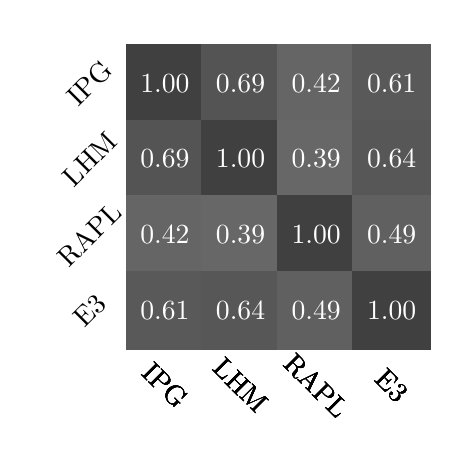
\begin{tikzpicture}[scale=0.6]
        \foreach \y [count=\n] in {{1.00, 0.69, 0.42, 0.61},{0.69, 1.00, 0.39, 0.64},{0.42, 0.39, 1.00, 0.49},{0.61, 0.64, 0.49, 1.00},} {
        % column labels
        \foreach \a [count=\n] in {IPG,LHM,RAPL,E3} {
          \node[minimum size=10mm, xshift=0.0cm, rotate=-45] at (\n*1.6, -8) {\a};
        }
        % heatmap tiles
        \foreach \x [count=\m] in \y {
          \pgfmathsetmacro{\xa }{(\x + 1) / 2 * 100}
          \node[fill=darkgray!\xa!lightgray, minimum size=10mm, text=white, font={\normalsize}] at (\m*1.6,-\n*1.6) {\x};
        }
      }
        % row labels
        \foreach \a [count=\i] in {IPG,LHM,RAPL,E3} {
          \node[minimum size=10mm, xshift=-0.0cm, yshift=-0.0cm, rotate=45] at (0,-\i*1.6) {\a};
        }
      \end{tikzpicture}
    \caption{This heat map represents Correlation coefficients between the different measurement instruments -1 to 1 on the Surface Pro 4}
    \label{tab:HeatFasta}
\end{figure}









% These results seem to indicate that all of the measuring instruments are correlated, which is expected as they measure the energy consumption of the same test cases, on the same DUT's. Another interesting thing to note here is that the correlation between the measurements on the workstation are higher as opposed to the two laptops as can be seen on \cref{tab:correlationWork,tab:CobineddCorrelation}. From this it can be seen that most of the measuring instruments are at least moderate correlated, except RAPL|E3.

%and this is especially true when looking at the workstation. %Another interesting observation is that all the measurements are less correlated on the laptops than the Workstation.




